\chapter{Introduction}

%Replace \lipsum with text.
% You may have as many sections as you please. This is just for reference.
Democracy is a system of government by all the eligible members of a state. In the words of Abraham Lincoln, it is \emph{the government of the people, by the people, for the people}.\\  

But from time to time, it has been observed that a democratic government can be loosely described in terms of a collection of \emph{ hegemonies } and \emph{counter hegemonies}. By a \emph{hegemony}, we actually mean the dominance over a society by people controlling important resources in the nation (natural or artificial) namely military, politics, academics, businesses, media etc. The distribution of power in hegemonic parties are often hereditary (among close ties in family) instead of elected representatives. Interactions among the persons of these important fields are also common for their effective functioning (or often to safeguard self-interests). \\

Yet the beauty of this system lies in the concept of \emph{counter hegemony} - a part of the civil society which functions to keep check on the hegemonic bodies. All the oppositions and protests against government and/or other powers, and such kind of information dispersion, comes under the flag of counter hegemony. To summarize, a democratic society can be said to controlled and influenced by these opposing forces of hegemony and counter-hegemony. \\

In this regard, accountability and transparency in government are the key requirements in order to obtain an ideal democratic society. Unfortunately the lack of proper knowledge about the \emph{power-houses} has led to new forms of \emph{collective} dictatorship where public rights and voices are sometimes rendered ineffective. \\

To account for this growing problem of opacity we have tried to study the social network of Indian politicians and corporates and disseminate the information to the common public through our present work.

% \textbf{Problem Statement} : Problem of forming the social networks of Indian Politicians and Corporates, visualizing  and analyzing them.

\section{Objective}
%\lipsum[1]

%You should cite papers in the following manner: Bayliss et al.~\cite{Bay1} gave an iterative method for Helmholtz equation etc.
%Similar work has been done in \cite{Bailey,Ernst,Gold3}.
The intent has been to complete the following tasks: 
\begin{itemize}

    %Todo remnove trhis???%

    \item To \textbf{collect data from semantic web} (and other sources) to form a database ( henceforth referred to as \textbf{"knowledge base"} / \textbf{"knowledge graph"} )
    
    \item To construct a \textbf{highly integrated, structured, error-free data store} by collecting and integrating political, corporate, bureaucratic and other kind of similar data which otherwise is scattered at random, dis-connected sources on the web.

    \item To provide \textbf{a data mash-up from different fields} to further help the academicians, journalists, data-enthusiasts etc.
    
    \item To \textbf{monitor the top players in Indian society} - mainly in the spheres of politics and business in India.
    
    \item To \textbf{disseminate this information to public} to bring about accountability and transparency. 
    
    \item  To seek answers to questions like -
        \begin{itemize}
         \item \emph{ Who were the big players in politics and business in the Indian domain? }
         \item \emph{ Is there any influence (or possibility of it) of political field by a person in corporate field or vice-versa? }
         \item \emph{ How important is one politician in a network of politicians (or a businessperson in a business network)? }
         \item \emph{ Where does the actual power reside in a democracy? }
        \end{itemize}
\end{itemize}
We believe that through our work, we will be able to show how such system of inter-disciplinary data helps to find interesting patterns and spread more knowledge.

\begin{figure}[H]
\begin{center}  
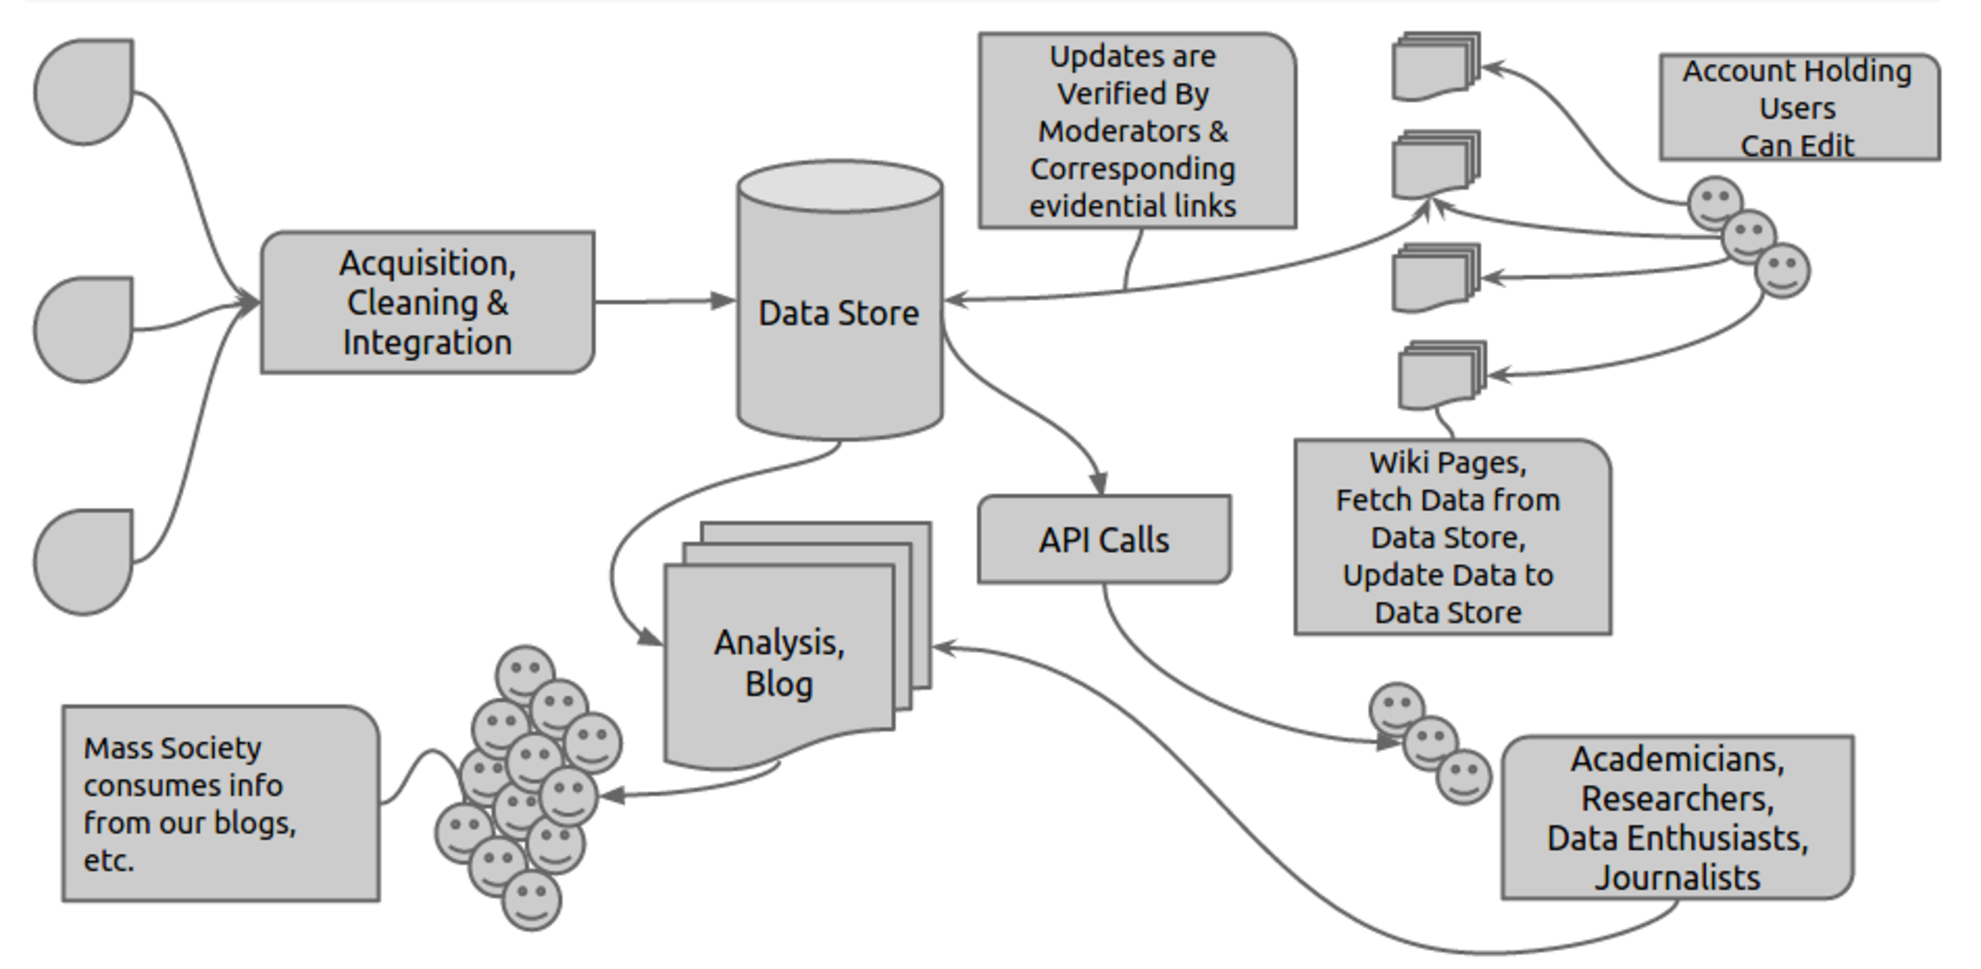
\includegraphics[width=1\textwidth]{big_pic} 
\caption{Big picture of the system envisioned}
\label{fig:big_pic}
\end{center}
\end{figure}

\section{Motivation \& Related Work}

In his book \textbf{The Power Elite} \cite{Mills}, C. Wright Mills calls attention to the interwoven interests of the leaders of the military, corporate, and political elements of society and suggests that the ordinary citizen is a relatively powerless subject of manipulation by those entities. His book deals with the power elite in US. But the hierarchy he proposes is more or less the same across all countries. Power rests with the top one percent in an economy. We plan to create a watchdog for that one percent. One interesting list to accompany this direction could be the Forbes list \cite{FORBES} of 147 companies that control everything. \\ 

French economist Thomas Piketty in his famous work \textbf{Capital in the Twenty-First Century} \cite{Piketty} focuses on wealth and income inequality in Europe and the United States since the beginning of the industrial revolution. He proposes a global system of progressive wealth taxes to help reduce inequality and avoid the vast majority of wealth coming under the control of a tiny minority. We plan to collect, integrate, visualize and open such data for Indian terrain to let data fanatics carry out such works to understand this inequality. \\

British writer and historian Patrick French, in his book \textbf{India: A Potrait} \cite{French} has stated many such interesting patterns in Indian politics where he argues that almost all of the young Indian politicians in the Indian Parliament are hereditary. In fact, patterns similar to this can be seen over the entire political Indian scene. One can find interesting overlaps, family ties, social links within these power houses. In a survey, \textbf{Who owns your media?} \cite{Media}, we find that even the media is an entity of importance in the game of power and most of the famous and powerful politicians and businessmen try to pull strings in this domain. Another interesting case is Jayant Sinha's family tree \cite{Sinha} and their business holdings. As of 2015, he was the Minister of State for Finance and a Member of Indian Parliament and had links to lot of powerful companies. \\

Research along the area have been prominent across countries. \textbf{Sastry} \cite{Sastry} shows how crime and money play important role in Indian elections. In a related work \textbf{Vaishnav} \cite{Essay} explain why do Indian parties elect criminal candidates and why they win. \textbf{Kapur} \cite{Builders} connects the hidden relationships between politicians and builders. He argues that where elections are costly but accountability mechanisms are weak, politicians often turn to private firms for illicit election finance and that where firms are highly regulated, politicians can exchange policy discretion or regulatory forbearance for bribes and monetary transfers from firms. \\

Works like what we propose have already been done for countries like USA, UK, Chile etc. We have examples like \textbf{LittleSis} \cite{LilSis}, \textbf{Poderopedia} \cite{PODERO} where journalists, developers, analysts come together to put up profiles of important entities, institutions of the society and highlighted the connections between them. Littlesis (opposite of Big brother) in one hand exists in USA from the political and economical data available there. Poderopedia is a similar site in Chile. These sites feature separate pages of people in power in USA, their connections to different institutions and other entities , work history, visualizations of the connections to educate masses etc. Other than producing awareness to people about the corporate- political connections, these sites also allow public to register and collaborate in data entry processes and have an API system to promote further use of their data for research purposes. \\

Such system in absence of digital data/ structured data and other human factors is difficult in India. But various local and national initiatives have been started. \textbf{Association for Democratic Reforms} \cite{ADR} for example has sites like \textbf{MyNeta} \cite{MyNeta} to disseminate information about political leaders of India. \\

Our vision is to produce a system similar in lines to the websites embedded with the power to query interesting connections, find interesting visualizations, and help raise suspicious issues. \\

The core two things that required our special attention when working with several data sources is the process of \textbf{ modeling the database as a graph } and method of \textbf{ resolving same entities from different data sources }. These two things are problems with extensive study of their own. \\

\textbf{ Entity resolution } has been studied since 1946 by works of \emph{ Halber.L.Dunn }\cite{dunn}. Basic method is to match a pair of strings accurately to determine possible similar entities. Since then, several string matching algorithms has been used for this purpose. The \textbf{levenshtein algorithm} \cite{levenshtein} gives score based on no of edits to convert one string to another. It is especially useful to deal with the problem of mis-spelt records. Improving on that the \textbf{Jaro-Winkler} \cite{jwinkler} looks at matching characters within a small range while giving scores. This is suitable for short strings such as names and fits our purpose well. Another class of string matching algorithms looks at phonetics to resolve entities with similar sounding text. The \textbf{ Soundex algorithm }\cite{knuth} is one of the most well known. These algorithms use English language pronunciations to create an index of the text. For our purpose, we have used the Jaro-Winkler and a variation of Soundex \textbf{ (Double Metaphone) }\cite{philips}. \\

    The graph model of the data is required since we are emphasizing the relationships among the data. Graph databases as a concept existed long since mid-1960s when \textbf{ IBM IMS } \cite{korth} \cite{ims} supported graph structures in its hierarchical model. Graph databases allow one to give semantic queries  over data relationships. A graph database models the entities as nodes and relationships among them as edges between nodes. Internally, a graph database stores the data as a relational table (\textbf{ MariaDB }\cite{maria}) or through document-value stores (\textbf{Neo4j, OrientDB}\cite{neo}\cite{orient}). For the purpose of our project we have used the Neo4j database to store the core-data. 

\section{Thesis Overview}
The rest of the work has been divided into following sections:

\begin{enumerate}
    
    \item \textbf{Constructing the Social Network} -  The choice of graph database has been explained here, with a detailed description of system's data model. The challenges and methods adopted while collecting and integrating data too have been described. Entity Resolution, which forms the basis of the entire system and which is one of the most important challenges of the work, has been discussed at length.
    
    \item \textbf{Design of Power Elites Web App}  -  A complete overview of the system is provided with all the possible actors. All the components  of the system, their functionalities and interactions with the actors of the system have been explained here. All the internal details of the wiki and how data is actually gathered and resolved is discussed thoroughly.

    \item \textbf{Visualizations and Analysis}- The results obtained from the constructed system have been described here. Interesting connections among and within the power houses have been listed here along-with the resultant observations. 

    \item \textbf{Conclusion and Further Work} - Various ways the present work can be expanded are listed here along with the conclusion of the work in hand. All important future additions and improvements have been documented.

\end{enumerate}
